% \documentclass[handout]{beamer}
\documentclass{beamer}

\mode<presentation>
{
  \usetheme{ANLBlue}
  % \usefonttheme[onlymath]{serif}
  % \usetheme{Singapore}
  % \usetheme{Warsaw}
  % \usetheme{Malmoe}
  % \useinnertheme{circles}
  % \useoutertheme{infolines}
  % \useinnertheme{rounded}

  \setbeamercovered{transparent=20}
}

\usepackage[english]{babel}
\usepackage[latin1]{inputenc}
\usepackage{alltt,listings,multirow,ulem,siunitx}
\usepackage[absolute,overlay]{textpos}
\TPGrid{1}{1}
\usepackage{pdfpages}
\usepackage{ulem}
\usepackage{multimedia}
\usepackage{multicol}
\newcommand\hmmax{0}
\newcommand\bmmax{0}
\usepackage{bm}
\usepackage{comment}
\usepackage{subcaption}

% font definitions, try \usepackage{ae} instead of the following
% three lines if you don't like this look
\usepackage{mathptmx}
\usepackage[scaled=.90]{helvet}
% \usepackage{courier}
\usepackage[T1]{fontenc}
\usepackage{tikz}
\usetikzlibrary{decorations.pathreplacing}
\usetikzlibrary{shadows,arrows,shapes.misc,shapes.arrows,shapes.multipart,arrows,decorations.pathmorphing,backgrounds,positioning,fit,petri,calc,shadows,chains,matrix,mindmap}

\newcommand\vvec{\bm v}
\newcommand\bvec{\bm b}
\newcommand\bxk{\bvec_0 \times \kappa_0 \cdot \nabla}
\newcommand\delp{\nabla_\perp}

% \usepackage{pgfpages}
% \pgfpagesuselayout{4 on 1}[a4paper,landscape,border shrink=5mm]

\usepackage{JedMacros}

\newcommand{\timeR}{t_{\mathrm{R}}}
\newcommand{\timeW}{t_{\mathrm{W}}}
\newcommand{\mglevel}{\ensuremath{\ell}}
\newcommand{\mglevelcp}{\ensuremath{\mglevel_{\mathrm{cp}}}}
\newcommand{\mglevelcoarse}{\ensuremath{\mglevel_{\mathrm{coarse}}}}
\newcommand{\mglevelfine}{\ensuremath{\mglevel_{\mathrm{fine}}}}

%solution and residual
\newcommand{\vx}{\ensuremath{x}}
\newcommand{\vc}{\ensuremath{\hat{x}}}
\newcommand{\vr}{\ensuremath{r}}
\newcommand{\vb}{\ensuremath{b}}

%operators
\newcommand{\vA}{\ensuremath{A}}
\newcommand{\vP}{\ensuremath{I_H^h}}
\newcommand{\vS}{\ensuremath{S}}
\newcommand{\vR}{\ensuremath{I_h^H}}
\newcommand{\vI}{\ensuremath{\hat I_h^H}}
\newcommand{\vV}{\ensuremath{\mathbf{V}}}
\newcommand{\vF}{\ensuremath{F}}
\newcommand{\vtau}{\ensuremath{\mathbf{\tau}}}


\title{Benchmarking Supercomputers}
\subtitle{This talk: \url{http://59A2.org/files/20141212-Benchmarking.pdf}}
\begin{comment}
The Top500 list has used a dense linear algebra benchmark (HPL) to rank
supercomputers since 1993.  Due to evolving hardware and algorithms,
performance on this benchmark is poorly correlated with that of real
applications, leading to boycotts by some prominent supercomputing
centers.  This talk will introduce principles of benchmark design,
characteristics of application performance, and hardware trends,
concluding with the new HPGMG benchmark that I have co-developed.
\end{comment}

\author{{\bf Jed Brown} \texttt{jed@jedbrown.org} (ANL and CU Boulder)}

% - Use the \inst command only if there are several affiliations.
% - Keep it simple, no one is interested in your street address.
% \institute
% {
%   Mathematics and Computer Science Division \\ Argonne National Laboratory
% }

\date{CU Boulder, 2014-12-12}

% This is only inserted into the PDF information catalog. Can be left
% out.
\subject{Talks}


% If you have a file called "university-logo-filename.xxx", where xxx
% is a graphic format that can be processed by latex or pdflatex,
% resp., then you can add a logo as follows:

% \pgfdeclareimage[height=0.5cm]{university-logo}{university-logo-filename}
% \logo{\pgfuseimage{university-logo}}



% Delete this, if you do not want the table of contents to pop up at
% the beginning of each subsection:
% \AtBeginSubsection[]
% {
% \begin{frame}<beamer>
%   \frametitle{Outline}
%   \tableofcontents[currentsection,currentsubsection]
% \end{frame}
% }

\AtBeginSection[]
{
  \begin{frame}<beamer>
    \frametitle{Outline}
    \tableofcontents[currentsection]
  \end{frame}
}

% If you wish to uncover everything in a step-wise fashion, uncomment
% the following command:

% \beamerdefaultoverlayspecification{<+->}

\begin{document}
\lstset{language=C}
\normalem

\begin{frame}
  \titlepage
\end{frame}

\begin{frame}{Why benchmark computers?}
  \begin{itemize}
  \item Justify purchases
  \item Superficial competition
  \item Help applications form realistic expectations
  \end{itemize}
\end{frame}

\begin{frame}{Why do we need an exascale computer?}
  \begin{itemize}
  \item Science \& engineering demands
    \begin{itemize}
    \item Model fidelity: resolution, multi-scale, coupling
    \item Inversion/data assimilation
    \item Optimization, control
    \item Quantify uncertainty, risk-aware decisions
    \item Sequence of forward simulations, each needing more time steps
    \end{itemize}
  \item External requirements on time-to-solution
    \begin{itemize}
    \item Policy: 5 SYPD for climate model to inform IPCC
    \item Weather: 250x faster than real-time
    \item Supply chain dynamics, manufacturing
    \item Field studies, disaster response
    \item Transient simulation is not weak scaling
    \end{itemize}
  \item ``weak scaling'' [\ldots] will increasingly give way to ``strong scaling''\\
    {\small [The International Exascale Software Project Roadmap, 2011]}
  \end{itemize}
\end{frame}

\begin{frame}{HPL and the Top500 list}
  \begin{center}
    \includegraphics[width=0.9\textwidth]{figures/Supercomputers-history.pdf}
  \end{center}
  \begin{itemize}
  \item High Performance LINPACK
  \item Solve $n\times n$ dense linear system: $\bigO(N^{3/2})$ flops on $N=n^2$ data
  \item Top500 list created in 1993 by Hans Meuer, Jack Dongarra, Erich
    Strohmeier, Horst Simon
  \end{itemize}
\end{frame}

\begin{frame}
  \includegraphics[width=\textwidth]{figures/karlrupp/flop-per-byte-dp.pdf} \\
  {\scriptsize [c/o Karl Rupp]}
\end{frame}

\begin{frame}{It's all about the memory}
  \begin{center}
    \includegraphics[width=.65\textwidth]{figures/Ang-CPUGPU.png}
    \includegraphics[width=.35\textwidth]{figures/Ang-AMDLlano.png} \\
    {\scriptsize [Ang et al, 2014]}
  \end{center}
  \begin{itemize}
  \item Memory motion dominates floating point cost
  \item About half of die devoted to caches
  \item Network moving on-die, maybe throughput cores
  \end{itemize}
\end{frame}

\begin{frame}{Algorithms keep pace with hardware (sometimes)}
  \includegraphics[width=\textwidth]{figures/KeyesAlgorithmsKeepPace.png} \\
  {\scriptsize [c/o David Keyes]}
  \begin{itemize}
  \item Opportunities now: uncertainty quantification, design
  \item Incentive to find optimal algorithms for more applications
  \end{itemize}
\end{frame}

\begin{frame}{What does ``representative'' mean?}
  \begin{itemize}
  \item Diverse applications
    \begin{itemize}
    \item explicit PDE solvers (seismic wave propagation, turbulence)
    \item implicit PDE solvers and multigrid methods (geodynamics, structural mechanics)
    \item irregular graph algorithms (network analysis, genomics, game trees) 
    \item dense linear algebra and tensors (quantum chemistry) 
    \item fast methods for N-body problems (molecular dynamics, cosmology) 
    \item cross-cutting: data assimilation, uncertainty quantification
    \end{itemize}
  \end{itemize}
\end{frame}

\begin{frame}{Necessary and sufficient}
  \begin{block}{Goodhart's Law}
    When a measure becomes a target, it ceases to be a good measure.
  \end{block}

  \begin{itemize}
  \item Features stressed by benchmark \textbf{necessary} for some apps
  \item Performance on benchmark \textbf{sufficient} for most apps
  \end{itemize}
\end{frame}

\begin{frame}{HPCG: High-Performance Conjugate Gradients}
  \begin{itemize}
  \item Heroux and Dongarra, 2013
  \item \url{http://hpcg-benchmark.org}
  \item Sparse matrices: 2 flops per 12 bytes
  \item Preconditioner depends on subdomain
  \item 50 iterations: asymptotically no progress toward solution
  \item Faux coarse grid -- only nearest neighbor dependencies
  \item Half the work computes known 0.0
  \item Goal defined by 2-norm versus $A$-norm
  \item User chooses problem size
  \end{itemize}
\end{frame}

\begin{frame}{Perverse cache effects}
  \begin{center}
    \includegraphics[width=0.75\textwidth]{figures/MarjanovicL3.png} \\
  \end{center}
  {\scriptsize [Marjanovi\'c, Gracia, Glass (2014)]}
  \begin{itemize}
  \item What rules to prevent this?
  \item on-package memory, DRAM, NVRAM
  \end{itemize}
\end{frame}

\begin{frame}{Does the network matter?}
  \begin{center}
    \includegraphics[width=0.75\textwidth]{figures/MarjanovicExtrapolating.png} \\
  \end{center}
  {\scriptsize [Marjanovi\'c, Gracia, Glass (2014)]}
  \begin{itemize}
  \item Nearest neighbor, some global reductions
  \end{itemize}
\end{frame}

\begin{frame}[fragile]{The gist of multigrid}
  \begin{figure}
    \centering
    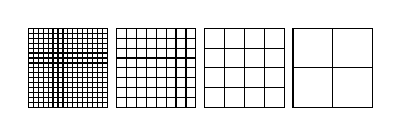
\begin{tikzpicture}
      [>=stealth,
      every node/.style={inner sep=2pt},
      restrict/.style={thick},
      prolong/.style={thick},
      mglevel/.style={rounded rectangle,draw=blue!50!black,fill=blue!20,thick,minimum size=4mm},
      ]
      \begin{scope}\scriptsize
        \newcommand\mgdx{4.0em}
        \newcommand\mgdy{4.0em}
        \newcommand\mgl[1]{(pow(2,#1+1))}
        \newcommand\mgloc[4]{(#1 + #4*\mgdx*#3,#2 + \mgdy*#3)}

        \newcommand\mghx{0.9*\mgdx}
        \newcommand\mghy{0.9*\mgdy}

        \draw[shift=\mgloc{0*\mgdx}{0}{0}{0},
        xstep=\mghy/\mgl{3},
        ystep=\mghy/\mgl{3}]
        (-0.5*\mghy,-0.5*\mghy) grid (0.5*\mghy,0.5*\mghy);

        \draw[shift=\mgloc{1*\mgdx}{0}{0}{0},
        xstep=\mghy/\mgl{2},
        ystep=\mghy/\mgl{2}]
        (-0.5*\mghy,-0.5*\mghy) grid (0.5*\mghy,0.5*\mghy);

        \draw[shift=\mgloc{2*\mgdx}{0}{0}{0},
        xstep=\mghy/\mgl{1},
        ystep=\mghy/\mgl{1}]
        (-0.5*\mghy,-0.5*\mghy) grid (0.5*\mghy,0.5*\mghy);


        \draw[shift=\mgloc{3*\mgdx}{0}{0}{0},
        xstep=\mghy/\mgl{0},
        ystep=\mghy/\mgl{0}]
        (-0.5*\mghy,-0.5*\mghy) grid (0.5*\mghy,0.5*\mghy);
      \end{scope}
    \end{tikzpicture}
    \label{fig:levels}
  \end{figure}
  \textbf{Multigrid} is an $O(n)$ method for solving algebraic problems by defining a hierarchy of scale.
  A multigrid method is constructed from:
  \begin{enumerate}
  \item a series of discretizations
    \begin{itemize}
    \item coarser approximations of the original problem
    \item constructed algebraically or geometrically
    \end{itemize}
  \item intergrid transfer operators
    \begin{itemize}
    \item residual restriction $I_h^H$ (fine to coarse)
    \item state restriction $\hat I_h^H$ (fine to coarse)
    \item partial state interpolation $I_H^h$ (coarse to fine, `prolongation')
    \end{itemize}
  \item Smoothers ($S$)
    \begin{itemize}
    \item correct the high frequency error components
    \item Richardson, Jacobi, Gauss-Seidel, etc.
    \end{itemize}
  \end{enumerate}
\end{frame}

\begin{frame}[fragile]
  \frametitle{Full Multigrid(FMG)}
  \begin{figure}
  \centering
  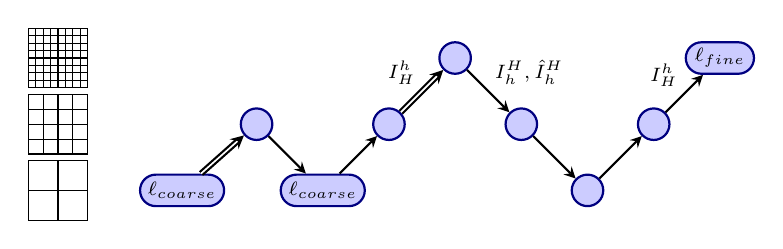
\begin{tikzpicture}
    [>=stealth,
    every node/.style={inner sep=2pt},
    restrict/.style={thick},
    prolong/.style={thick},
    mglevel/.style={rounded rectangle,draw=blue!50!black,fill=blue!20,thick,minimum size=4mm},
    ]
    \begin{scope}\scriptsize
      \newcommand\mgdx{3.0em}
      \newcommand\mgdy{3.0em}
      \newcommand\mgl[1]{(pow(2,#1+1))}
      \newcommand\mgloc[4]{(#1 + #4*\mgdx*#3,#2 + \mgdy*#3)}

      \node[mglevel] (coarseinit) at \mgloc{-3}{0}{0}{0} {$\mglevel_{coarse}$};

      \node[mglevel] (afine) at \mgloc{0}{0}{1}{1} {};

      \node[mglevel] (bcoarse) at \mgloc{2*\mgdx}{0}{0}{1} {$\mglevel_{coarse}$};
      \node[mglevel] (bup1) at \mgloc{2*\mgdx}{0}{1}{1} {};
      \node[mglevel] (bfine) at \mgloc{2*\mgdx}{0}{2}{1} {};

      \node[mglevel] (cdown1) at \mgloc{6*\mgdx}{0}{1}{-1} {};
      \node[mglevel] (ccoarse) at \mgloc{6*\mgdx}{0}{0}{-1} {};
      \node[mglevel] (cup1) at \mgloc{6*\mgdx}{0}{1}{1} {};
      \node[mglevel] (cfine) at \mgloc{6*\mgdx}{0}{2}{1} {$\mglevel_{fine}$};


      \draw[->,restrict,double]
                         (coarseinit) -- node [above right] {} (afine);
      \draw[->,restrict]
                         (afine) -- node [above right] {} (bcoarse);
      \draw[->,restrict]
                         (bcoarse) -- node [above right] {} (bup1);
      \draw[->,restrict,double]
                         (bup1) -- node [above left] {$\mathbb I_H^h$} (bfine);
      \draw[->,restrict]
                         (bfine) -- node [above right] {$I_h^H,\hat I_h^H$} (cdown1);
      \draw[->,restrict]
                         (cdown1) -- node [above right] {} (ccoarse);
      \draw[->,restrict]
                         (ccoarse) -- node [above right] {} (cup1);
      \draw[->,restrict]
                         (cup1) -- node [above left] {$I_H^h$} (cfine);

      %grids
      \newcommand\mghx{0.9*\mgdx}
      \newcommand\mghy{0.9*\mgdy}

      \draw[shift=\mgloc{-2*\mgdx}{0}{2}{0},
      xstep=\mghy/\mgl{2},
      ystep=\mghy/\mgl{2}]
      (-0.5*\mghy,-0.5*\mghy) grid (0.5*\mghy,0.5*\mghy);

      \draw[shift=\mgloc{-2*\mgdx}{0}{1}{0},
      xstep=\mghy/\mgl{1},
      ystep=\mghy/\mgl{1}]
      (-0.5*\mghy,-0.5*\mghy) grid (0.5*\mghy,0.5*\mghy);

      \draw[shift=\mgloc{-2*\mgdx}{0}{0}{0},
      xstep=\mghy/\mgl{0},
      ystep=\mghy/\mgl{0}]
      (-0.5*\mghy,-0.5*\mghy) grid (0.5*\mghy,0.5*\mghy);

  \end{scope}
\end{tikzpicture}
\label{fig:FMG}
\end{figure}
\begin{itemize}
  \item start with coarse grid
  \item truncation error within one cycle
  \item about five work units for many problems
  \item no ``fat'' left to trim
\end{itemize}
\end{frame}

\begin{frame}{HPGMG: a new benchmarking proposal}
  \begin{itemize}
  \item \url{https://hpgmg.org}, hpgmg-forum@hpgmg.org mailing list
  \item Mark Adams, Sam Williams (finite-volume), Jed (finite-element), John Shalf, Brian Van Straalen, Erich Strohmeier, Rich Vuduc
  \item Gathering momentum, SC14 BoF
  \item Implementations
    \begin{description}
    \item[Finite Volume] memory bandwidth intensive, simple data dependencies
    \item[Finite Element] compute- and cache-intensive, vectorizes, overlapping writes
    \end{description}
  \item Full multigrid, well-defined, scale-free problem
  \item Matrix-free operators, Chebyshev smoothers
  \end{itemize}
\end{frame}

\begin{frame}{Kiviat diagrams}
  \begin{center}
    \includegraphics[width=\textwidth]{figures/hpgmg-kiviat-20140606.png}
  \end{center}
  \begin{itemize}
  \item c/o Ian Karlin and Bert Still (LLNL)
  \end{itemize}
\end{frame}

\begin{frame}{How much parallelism out of how much cache?}
  \begin{tabular}{l rrrr rr}
    \toprule
    Processor & v width & threads & F/inst & latency & L1D & L1D/\#par \\
    \midrule
    Nehalem & 2 & 1 & 2 & 5 & 32 KiB & 1638 B \\
    Sandy Bridge & 4 & 2 & 2 & 5 & 32 KiB & 819 B \\
    Haswell & 4 & 2 & 4 & 5 & 32 KiB & 410 B \\
    BG/P & 2 & 1 & 2 & 6 & 32 KiB & 1365 B \\
    BG/Q & 4 & 4 & 2 & 6 & 32 KiB & 682 B \\
    KNC & 8 & 4 & 4 & 5 & 32 KiB & 205 B \\
    Tesla K20 & 32 & * & 2 & 10 & 64 KiB & 102 B \\
    \bottomrule
  \end{tabular}
  \begin{itemize}
  \item Most ``fast'' algorithms do about $O(n)$ flops on $n$ data
  \item DGEMM and friends do $O(n^{3/2})$ flops on $n$ data
  \item Exploitable parallelism limited by cache and register load/store
  \item L2/L3 performance highly variable between architectures
  \end{itemize}
\end{frame}

\begin{frame}{SuperMUC (FDR 10, E5-2680)}
  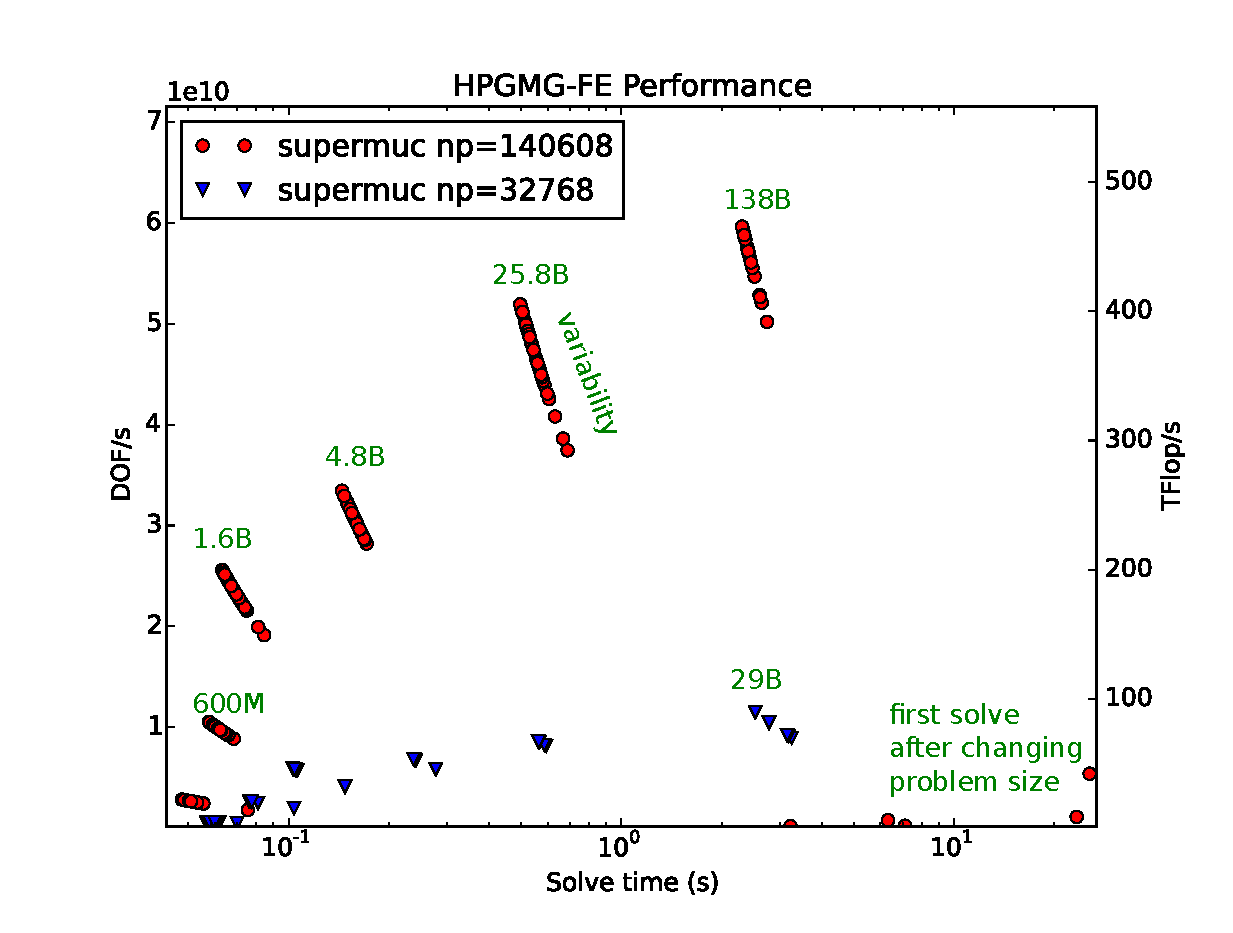
\includegraphics[width=\textwidth]{figures/hpgmg/range-supermuc-ann.eps}
\end{frame}

\begin{frame}{Edison (Aries, E5-2695v2)}
  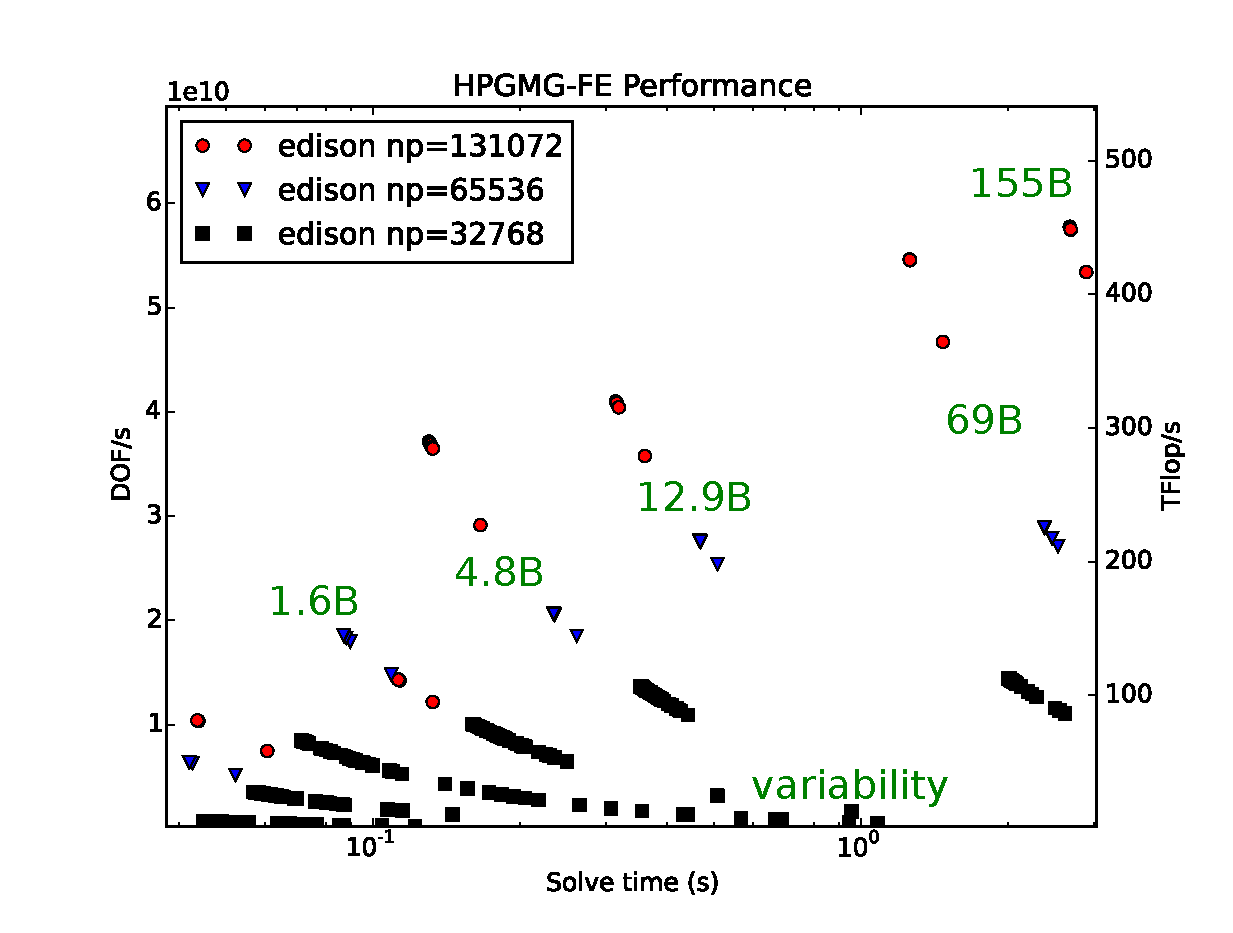
\includegraphics[width=\textwidth]{figures/hpgmg/range-edison-ann.eps}
\end{frame}

\begin{frame}{Edison, SuperMUC, Titan}
  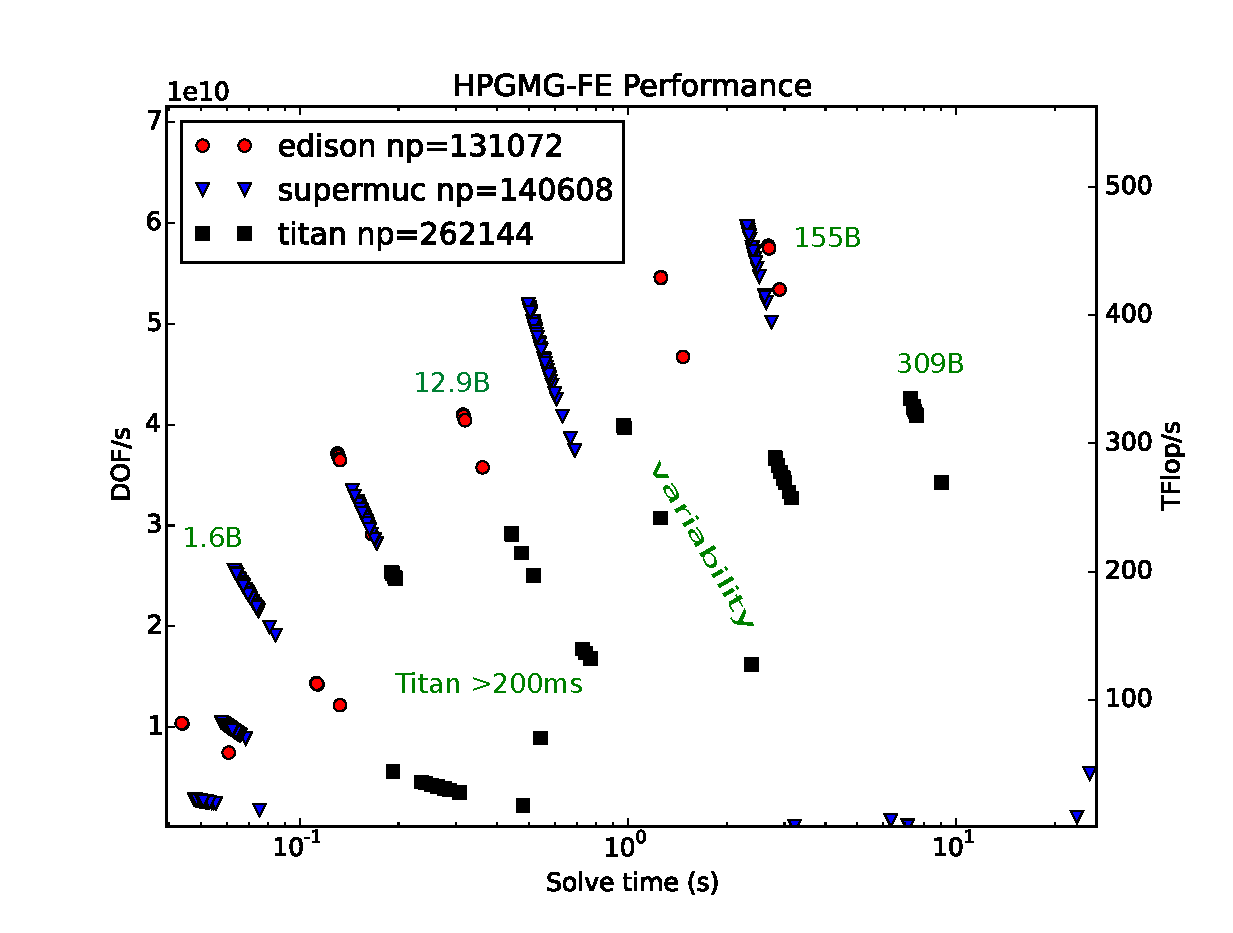
\includegraphics[width=\textwidth]{figures/hpgmg/range-edison-supermuc-titan-ann.eps}
\end{frame}

\begin{frame}{HPGMG distinguishes networks at 1M dofs/core}
  \begin{center}
    \includegraphics[width=0.6\textwidth]{figures/hpgmg-fv-20140515-dof.png}
  \end{center}
  \begin{itemize}
  \item Peregrine and Edison have identical node architecture
  \item Peregrine has 5:1 tapered IB, Edison has Aries dragonfly topology
  \end{itemize}
\end{frame}

\begin{frame}{MIC communication bottlenecks on Stampede}
  \begin{center}
    \includegraphics[width=\textwidth]{figures/hpgmg/fv-mic-mpi.png}
  \end{center}
\end{frame}

\begin{frame}{Outlook}
  \begin{itemize}
  \item What is the cost of performance variability?
  \item Finite element or finite volume?
    \begin{itemize}
    \item overlapping writes, cache reuse
    \item FE: $>20\%$ Intel, $6\%$ Blue Gene/Q; vs $10\%$ for FV
    \end{itemize}
  \item Linear or nonlinear?
  \item Irregularity and adaptivity
  \item Should dynamic range enter into the metric?
  \end{itemize}
\end{frame}

\begin{frame}{HPC Performance Modeling and Analysis}
  \begin{itemize}
  \item Spring 2015, Special Topics
  \item Architectural roadmaps and modeling
  \item Performance variability
  \item Designing performance experiments
  \item Application case studies
  \item Target audience:
    \begin{itemize}
    \item Advanced undergraduate and graduate students in Computer Science
    \item Graduate students in simulation-based science or engineering
    \end{itemize}
  \item \url{jed@jedbrown.org}
  \end{itemize}
\end{frame}

\end{document}
